%!TEX root = ../paper.tex
\section{Concept}
\label{sec:concept}

We now present our approach to the \nto problem.
The next section details our two-staged classification approach.
We then talk about what features we select and how we approach the \emph{\documentmismatch}.

\subsection{Two-staged classification}
As presented in Section~\ref{sec:background-problem} there exist two different concepts within a user's post.
These concepts are orthogonal to each other, as shown below.

First, users might express a need, demand, or interest for some product or not.
This might be a product of our company or not.
Typical phrases, taken from an experiment on our example data set (see Section~\ref{sec:evaluation}), for this concept are:
\begin{center}
	\textit{need, hi, looking for, recommend, please, anyone, appreciate, thank you}
\end{center}
We call this the \emph{demand classification}:
\begin{align}
	\mathbf{demand}&: POSTS \longrightarrow \big\{ ``demand", ``no-demand" \big\}
\end{align}

The second concept is about which product the user is talking about in the post.
Here, the decision needs to be made whether this is a product of the company or not.
In the latter case, we are not interested in the post anymore.
Depending on the actual product, the relevant words vary greatly.
The following words are relevant words for a customer relationship managment software, also taken from our example data:
\begin{center}
	\textit{customer, sales, crm, b2b, consumer, salesforce, organization, account}
\end{center}

We call this the \emph{product classification}:
\begin{align}
	\mathbf{product}&: POST \longrightarrow  PRODUCT \cup \big\{ NONE \big\}, \\
\end{align}

The intersection of the most relevant words for demand and product classification is the empty set.
This shows, that these concepts are independent of each other and should be treated separately.
Therefore, we split the \nto problem in two subproblems: given a post $p \in POSTS$ we first identify, whether the posts expresses a demand for a product.
If this is true, we then check whether we can actually categorize the post into one of our product groups.
All together, given $demand$ and $product$, we can define \nto:
\begin{alignat*}{3}
  &\mathbf{NTO}: && ~POSTS && \longrightarrow PRODUCT \cup \big\{ NONE \big\} \\
  &\mathbf{NTO}: && ~~p   && \longmapsto \begin{cases}
	    product(post)~~~~~~~\text{if }~demand(post) = ``demand" \\
	    NONE~~~~~~~~~~~~~~~\text{otherwise}
   \end{cases}
\end{alignat*}

In our system, both $demand$ and $product$ are implemented by two independent text classification algorithms.
We are using supervised machine learning for this.
Supervised learning requires tagged training samples to draw conclusions on unseen test samples.

The training data for the $demand$ classifier comes from manually classified demand posts.
However, the demand classification does not change for different companies or products.
It is independent from the product classification, which is why companies do not need to supply training data for the demand classification.
Rather, they can use a prebuild demand classifier.

The training data for the $product$ classifier needs to be supplied in form of brochures and/or marketing material for the different products.
Each brochure must be assigned to one product.
The system then automatically learns from the brochures.
Figure~\ref{fig:workflow} illustrates the architecture of the system.

\begin{figure}
	\label{fig:workflow}
	\begin{center}
		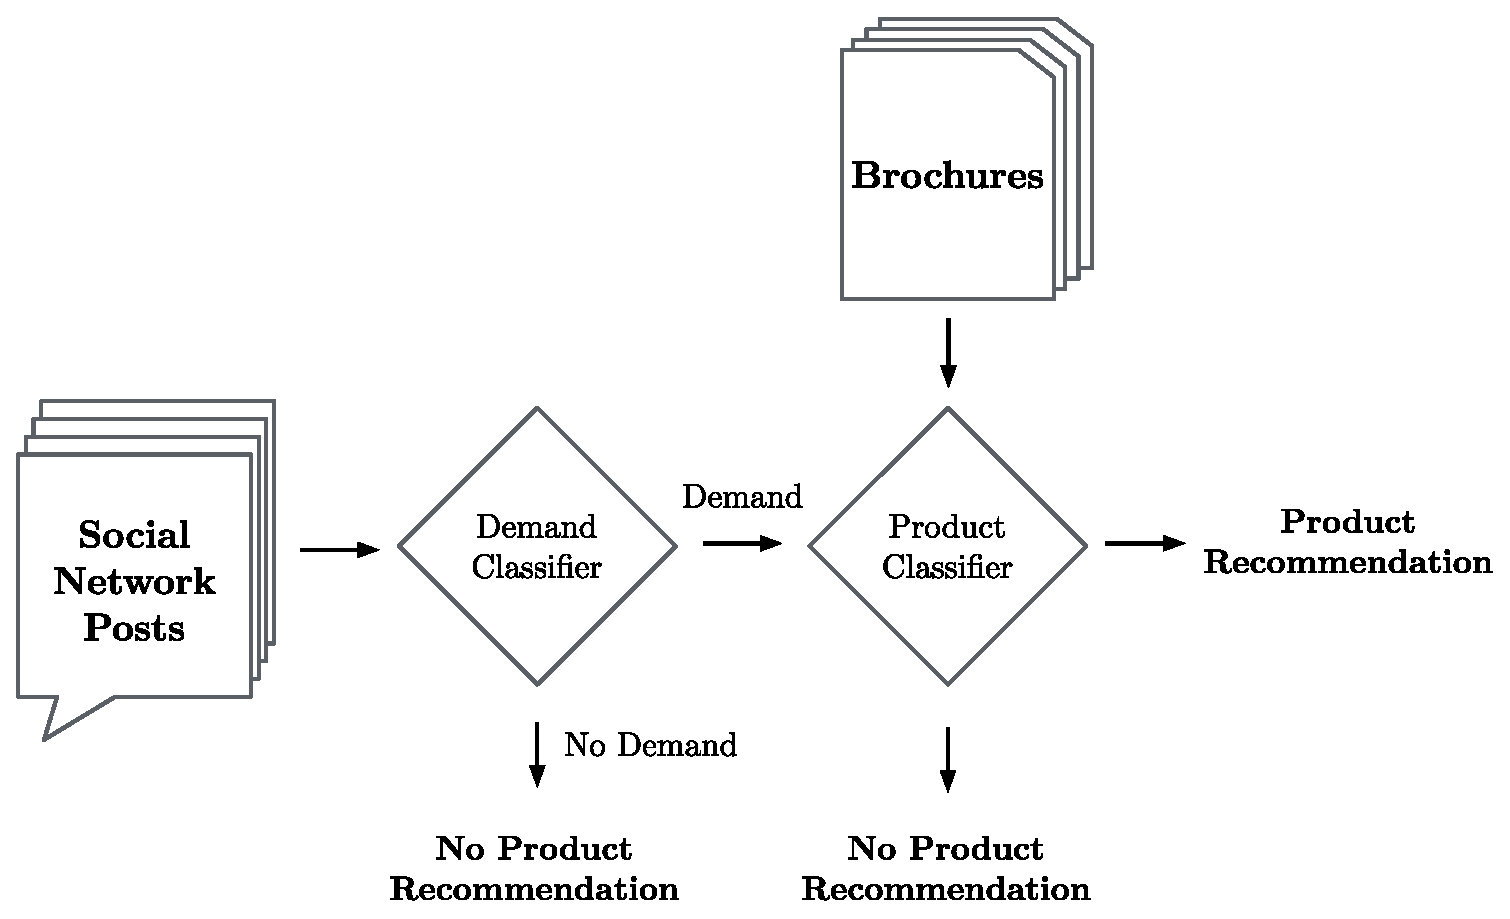
\includegraphics[width=0.7\textwidth]{figures/nto_workflow.eps}
	\end{center}
	\caption{Together, a demand classifier training from social network posts and a product classifier trained from marketing material form a classification-model for unseen posts.}
\end{figure}


Learning these two concepts with different classifiers also helps over come data sparsity issues.
The number of posts that actually are asking for a product of the company is low.
In our example data set, these posts only cover \todo{XX}~\% of the posts, whereas demand posts occur with \todo{XX}~\% probabilty and product documents with \todo{XX}~\%.
If the machine learning would work \cite{monard2002learning}.
This allows to get better results with fewer training data.

Only a few training data
Different characteristica
Example: Demand aber kein PRoduct
Schnittmenge der charakteristischen worte sehr klein
Schnittmenge der eigentlichen Dokumente auch sehr klein (only few positive examples)

only a few 

\begin{itemize}
	\item Two-staged classifier (why we did this)
	\item Feature selection
	\item Training data generation (using splits and random recombinations)
\end{itemize}

% \begin{itemize}
% 	\item Elaborate on your idea
% 	\item First give examples and than try to generalize
% \end{itemize}

\begin{figure}
	\centering
	\begin{subfigure}[t]{0.3\textwidth}
		\begin{tabular}{r | r}
			\textbf{Threads} & \textbf{Runtime}\\
			\hline
			1 & 29952\\
			2 & 15538\\
			4 & 10467\\
			8 & 7987
		\end{tabular}
		\caption{Computation of keyword distribution and identification of bursty intervals}
	\end{subfigure}~
	\begin{subfigure}[t]{0.3\textwidth}
		\begin{tabular}{r | r}
			\textbf{Threads} & \textbf{Runtime}\\
			\hline
			1 & 4649\\
			2 & 4430\\
			4 & 5429\\
			8 & 6427
		\end{tabular}
		\caption{Creation of events from keyword clustering}
	\end{subfigure}~
	\begin{subfigure}[t]{0.3\textwidth}
		\begin{tabular}{r | r}
			\textbf{Threads} & \textbf{Runtime}\\
			\hline
			1 & 514\\
			2 & 281\\
			4 & 250\\
			8 & 203
		\end{tabular}
		\caption{Matching of documents to events}
	\end{subfigure}
	\caption{Performance of each step of the algorithm in dependence of the number of threads employed}
	\label{fig:scalability}
\end{figure}
